\documentclass[a4paper]{article}

\usepackage{amsmath}
\usepackage{array}
%\usepackage{showframe}

\usepackage{tikz}

\newcommand{\ftri}[3]{
\begin{tikzpicture}[scale=2, baseline=(t.base)]
  \node[label={[shift={(0, -1.6)}]\Huge #1}] (t) at (1, 1.73) {};
  \node[label={[shift={(1.2, 0.3)}]\Huge #2}] (l) at (0, 0) {};
  \node[label={[shift={(-1.2, 0.3)}]\Huge #3}] (r) at (2, 0) {};
  \draw[black,thick] (l.center) -- (r.center) -- (t.center) -- (l.center);
  \draw (0.5, .865) -- (1.5, 0.865);
  \draw (1.0, .865) -- (1.0, 0);
\end{tikzpicture}
}

\begin{document}


\begin{tikzpicture}[scale=0.5]
\foreach \r in {5,4,...,0}{
\draw[fill=red,draw=black] (0,0) circle[radius=\r+0.5];
\draw[fill=white,draw=black] (0,0) circle[radius=\r];
};
\end{tikzpicture}

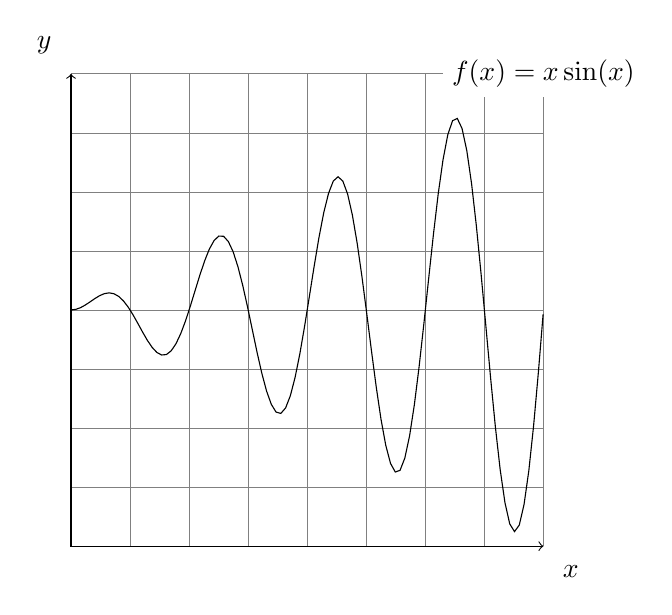
\begin{tikzpicture}[scale=3]
\node[label=above left:$y$] (topLeft) at (0, 2) {};
\node[label=below right:$x$] (botRight) at (2, 0) {};
\draw[step=0.25,gray,very thin] (0,0) grid (2,2);
\draw[<->] (topLeft.center) -- (0, 0) -- (botRight.center);
\draw[domain=0:2,fill=none,samples=100,draw=black]
plot (\x, {\x*sin(2*360*\x)/2 + 1});
\node[fill=white] at (2, 2) {$f(x) = x \sin(x)$};
\end{tikzpicture}

\ftri{V}{I}{R}

\begin{tabular}{| c | m{5cm} |} \hline
  \textbf{Formula} & \textbf{Explanation} \\ \hline
  \ftri{V}{I}{R}   & Electrical resistance is the ratio of p.d. applied to current flowing \\ \hline
  \ftri{F}{m}{a}   & Force applied is the product of mass and acceleration produced \\ \hline
\end{tabular}

\end{document}
